%!TEX root = ../template.tex
%Developed using Sublime Text 3 with LaTexTools plugin
%SUPER+b for compiling latex to pdf
%Don't forget to use SUPER+R to jump between top level commands!
%F6 to spell check
%%%%%%%%%%%%%%%%%%%%%%%%%%%%%%%%%%%%%%%%%%%%%%%%%%%%%%%%%%%%%%%%%%%%
%% chapter4.tex
%% UNL thesis document file
%%
%% Chapter with the info about the available data
%%%%%%%%%%%%%%%%%%%%%%%%%%%%%%%%%%%%%%%%%%%%%%%%%%%%%%%%%%%%%%%%%%%%
\chapter{Proposed Approach}
\label{cha:available_data}
% ================
% = Introduction =
% ================

For this dissertation's work, it's proposed a CRISP-DM methodology to approach the problem. An explanation about this methodology is presented in section \ref{sec:crispdm}, following a suggested working plan for this dissertation in section \ref{sec:work_plan}. In section \ref{sec:available_data} the available data is presented and its quality is discussed, referring that an additional dataset is expected.

As off the time this document is being written, the Business Understanding phase has already finished and the current focus is on the Data Understanding and the Data Preparation.

\todo[inline]{na parte de utilização das tecnicas, ser mencionado de forma suave o que é cada técnica}



\section{Cross Industry Standard Process for Data Mining} % (fold)
\label{sec:crispdm}

\Acrfull{crispdm} is an iterative data mining process model that describes commonly used approaches that data mining experts use to tackle problems, which was developed by analysts representing Daimler-Chrysler, SPSS, and NCR. \Acrshort{crispdm} provides a nonproprietary and freely available standard process for fitting data mining into the general problem-solving strategy of a business or research unit.

In this methodology, a data mining project has a life-cycle consisting in six phases, where the next phase in the sequence often depends on the outcomes associated with the previous phase - making it an adaptive methodology, where the sequence of the phases is not strict and moving back and forth between different phases is always required.

The iterative nature of \Acrshort{crispdm} provides a continuous approach for cases when the solution to a particular business or research problem leads to further questions of interest, which may then be attacked using the same general process as before.


\begin{figure}[htbp]
	\centering
	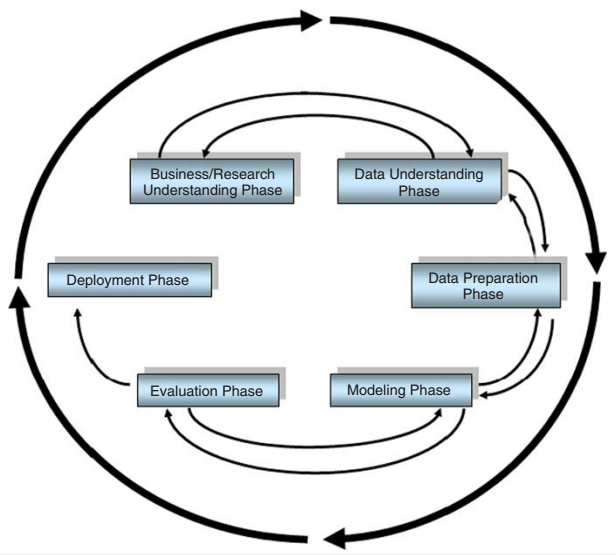
\includegraphics[width=4.5in ]{crispdm}
	\caption{\Acrshort{crispdm} process}
	\label{fig:crispdm}
\end{figure}

\subsection{CRISP-DM phases}
\label{subsec:crispdm_phases}

\subsubsection{Business/Research Understanding}
\label{subsubsec:business_understanding}

This initial phase focuses on clearly enunciate the project objectives and requirements in terms of the business or research unit as a whole. Then, it is necessary to convert this knowledge into a data mining problem definition, so that a preliminary strategy is made for achieving these objectives.

\subsubsection{Data Understanding}

This phase starts with the collection of the data to proceed with activities in order to get familiar with the data. The next step is evaluate the quality of the data and get the firsts insights. Finally, if desired, interesting subsets can be selected that may contain actionable patterns to form hypotheses for hidden information.

\subsubsection{Data Preparation}

This labor-intensive phase covers all aspects of preparing the final data set, which shall be used for subsequent phases, from the initial raw data. Data preparation tasks are prone to be performed multiple times, and not in any prescribed order. Tasks include selecting cases and variables to analyse, perform transformations on certain variables, and clean the raw data so that it is ready for the modeling tools.

\subsubsection{Modeling}

In this phase, the goal is to select and apply appropriate modeling techniques for further parameters' calibration to optimal value. Typically, several techniques may be applied for the same data mining problem. Some techniques have specific requirements on the form of data. Therefore, looping back to data preparation phase is often required.

\subsubsection{Evaluation}

At this stage in the project you have built a model (or models) that were delivered from Modeling phase. These models must be evaluated for quality and effectiveness, before they can be deploy for use in the field.
Before the deployment, it is also necessary to determine whether the model in fact achieves the objectives set for it in phase \ref{subsubsec:business_understanding}. Another key objective in this phase is to establish whether some important business issue has not been sufficiently accounted for. At the end of this phase, a decision on the use of the data mining results should be reached.

\subsubsection{Deployment}

Although this is the last phase, the creation of the model is generally not the end of the project. Depending on the requirements, the deploy can be as simple as generating a report or as complex as implementing a repeatable data scoring or data mining process. For businesses, the customer often carries out the deployment based on the analyst model.


\section{Work Plan} % (fold)
\label{sec:work_plan}

According to the CRISP-DM methodology, the first phase of this dissertation consisted on the study of three phase circuits and \acrshort{ims}, as well as understanding the several problems that affect them and the associated state of the art. The output of this phase consists on a document where the basics of three phase circuits can be learned from the perspective of a Computer Scientist, plus the problem definition which this dissertation is approaching. The next steps consist on data preparation and modeling, where an iterative approach will be done by interweaving the study of Signal Processing (\ref{subsec:data_prep_studying_signal}) and Machine Learning techniques (\ref{subsec:modeling_under_machine_learning}). 
After the experience and knowledge acquired through phase \ref{subsec:data_prep_studying_signal} and \ref{subsec:modeling_under_machine_learning} using a specific dataset, the modeling phase is expected to be re-iterated since a new dataset is expected by September. Meanwhile, an evaluation of the most promising models will be made. Although the process may be re-iterated, a prototype is expected as a result of this dissertation work.


\subsection{Understanding Induction Motors}

A focused output of this phase is summarise on chapter \ref{cha:intro_electric_motors}, where an understanding of the target motor in this dissertation can be found. A more complete output of this phase can be found on a future appendix of this document.


\subsection{Data Understanding}

At the moment, two datasets are available. One of the datasets can't be used since the sample rate of the metrics is too big to detected small fluctuations on the current to detect inter-turn short circuit between a low number of turns.
The other dataset is divided in 3 categories: healthy motor samples, faulty motor samples with 2 turns short-circuited, and faulty motor samples with 19 turns short-circuited. Its sample frequency is appropriate to detect such faults, but the sample period is merely 4 seconds long for each category and therefore doesn't have statical relevance on the lifetime of the motor. Therefore, this dataset is useful to understand the data as well as to understand the transformation that can be applied to get more insights.
It is expected that more data will be collected from several motors starting September. A more detailed section on this subject can be found on \ref{sec:available_data}.

\subsection{Data Preparation: Understanding Signal Processing}
\label{subsec:data_prep_studying_signal}

This phase will proceed in parallel with phase \ref{subsec:modeling_under_machine_learning}. Given the features available in the raw data, it is necessary to derive another set of features so that the differences between healthy stream data and faulty stream data can be found. Since the data is the representation of several signals (voltage and current), emerges the necessity to study several techniques to analysis this kind of data. For this purpose, a set of Signal Processing techniques will be study such as Fourier Analysis, several transforms (Hilbert, Laplace, Z, Fourier), as well as several signal filters.
The transform to study where chosen given its use in several relevant works ~\cite{M.a2014} ~\cite{Riera-Guasp2015} ~\cite{Cheng2011} and its relevance in the classical signal processing.
The goal is to try some features addition on the data and test some modeling techniques, while studying a specific signal processing technique and data streaming methods.


\subsection{Modeling: Understanding Machine Learning Techniques}
\label{subsec:modeling_under_machine_learning}

This phase will proceed in parallel with phase \ref{subsec:data_prep_studying_signal}. As an result of the state of the art's study, several works use Artificial Neural Networks and Support Vector Machines to detect faults ~\cite{Toma2011} ~\cite{Wolkiewicz2013} ~\cite{Patel2016} ~\cite{Jagadanand2015}. Therefore, these machine learning techniques will be study for further modeling. While developing the models, they will also be evaluated and compared with each others.  
Other techniques that will be studied are Clustering techniques.

\subsubsection{Artificial Neural Networks}

Artificial neural networks (ANN) are classifiers inspired by Biology. As all kind of classifiers, an ANN goal is to maximize the likelihood for the predicted result of a given input to be as close as possible of the real result. This goal is accomplished by training the ANN , which will adapt the consideration of the input against the expected result of that input. This classifier provides a general method for learning functions from examples, being the examples real-valued, discrete-valued, or vector-valued.

ANN are composed by perceptrons, which are units that take a vector of real-valued inputs, calculates a linear combination of these inputs, and then computes a function which will give the result, as seen in figure \ref{fig:sigmoid_unit}.

\begin{figure}[htpb]
\centering
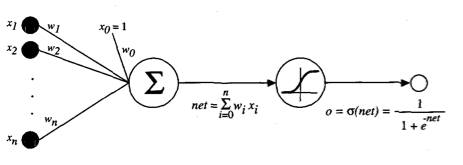
\includegraphics[width=0.5\textwidth]{sigmoidunit.png}
\caption{A perception unit with sigmoid activation function}
\label{fig:sigmoid_unit}
\end{figure}

Each perceptron have a linear combination so that a value may be produced from the input vector. from figure \ref{fig:sigmoid_unit}, it can be seen that each input has its own height. So, for example, a simple linear combination could be such as the equation \ref{eq:linear_combination}.

\begin{equation} 
\label{eq:linear_combination}
\sum_{i=1}^{n} w_{i}*x_{i}
\end{equation}

After the perceptron computes the linear combination, this value is applied to a function which will give us the class. For example, in a binary classification problem, the activation function can be the Logistic Function - also called sigmoid function.

\subsubsection{Support Vector Machine}

\subsection{New dataset acquisition and Modeling re-iteration}
\label{subsec:reiteration}

The new dataset will have a superset of the currently working dataset's features. Therefore, it is expected that the knowledge gained in previous phases will be valid to used and it's expected that the same input features will be used, but now the model will have a more statistical significant sample. More info about the new dataset can be found in section \ref{sec:available_data}.


\section{Available Data}
\label{sec:available_data}
